\sect{Evaluación}{evaluacion}

Para evaluar la usabilidad de la aplicación, se ha realizado una encuesta a varios usuarios seleccionados.
Esta se ha realizado a través de la herramienta \boldFont{Tally.so}, que permite crear encuestas de manera
sencilla y obtener los resultados de una forma visual.

El objetivo principal de esta encuesta es obtener una
valoración de la aplicación en cuanto a su usabilidad, así como obtener información sobre los aspectos que se pueden
mejorar y errores que no se hayan detectado en la fase de desarrollo.

Al inicio de la encuesta se recomienda al usuario que utilice la versión para ordenador de la aplicación, ya que
es la que se ha desarrollado y probado durante el proyecto.\ También se muestra una breve explicación del funcionamiento
de la aplicación, para que el usuario pueda realizar la encuesta de manera más sencilla.\ Además, el usuario debe
tener la sesión iniciada para poder completar la encuesta.\ Las preguntas que se incluyen en la encuesta son las
siguientes:

\begin{itemize}
	\item \boldFont{¿La interfaz es sencilla de utilizar?} - Es una escala de 1 a 5, donde 1 es
	\textit{Nada sencilla} y 5 es \textit{Muy sencilla}.
	\item \boldFont{¿Los pasos del cuestionario han sido fáciles de seguir?} - Respuesta igual que la anterior.
	\item \boldFont{¿Qué navegador has utilizado?} - Respuesta de selección entre varias opciones:
	\begin{itemize}
		\item Google Chrome.
		\item Mozilla Firefox.
		\item Brave.
		\item Opera.
		\item Microsoft Edge.
		\item Safari.
		\item Otro.\ En este caso, se pide que se especifique cuál.
	\end{itemize}
	Esto permite conocer qué navegadores son los más utilizados por los usuarios y si la aplicación funciona
	correctamente en todos ellos.
	\item \boldFont{Menciona lo que te gustaría que la aplicación mejorase.}
	\item \boldFont{Escribe lo que te gustaría ver añadido en un futuro en la aplicación.}
	\item \boldFont{¿Has encontrado algún error? Aquí puedes escribir cómo se puede reproducir el fallo (o adjuntar
	una imagen) para corregirlo en la siguiente versión de la aplicación.}

	Las últimas tres preguntas son de tipo abierto, para que el usuario pueda escribir lo que considere oportuno.
	En el caso de la última pregunta, además se permite adjuntar imágenes (o vídeos) para que el usuario pueda mostrar
	el error que ha encontrado y cómo se puede reproducir.\ De esta manera, se puede corregir el error conociendo
	con precisión el punto de fallo.\ El enlace a la encuesta se puede encontrar en el
	anexo~\ref{anx:encuesta-satisfaccion}.

	Para mostrar algunos datos recogidos en la encuesta se han realizado capturas de pantalla a algunas respuestas,
	que son totalmente anónimas, y se muestran a continuación:

	\begin{figure}[h]
		\centering
		\includegraphics[width=\textwidth]{res/images/Recuento de Qué navegador has utilizado}
		\caption{Recuento de la pregunta \textit{¿Qué navegador has utilizado?} (Fuente: Elaboración propia).}
		\label{fig:recuento-navegador}
	\end{figure}

	\begin{figure}[h]
		\centering
		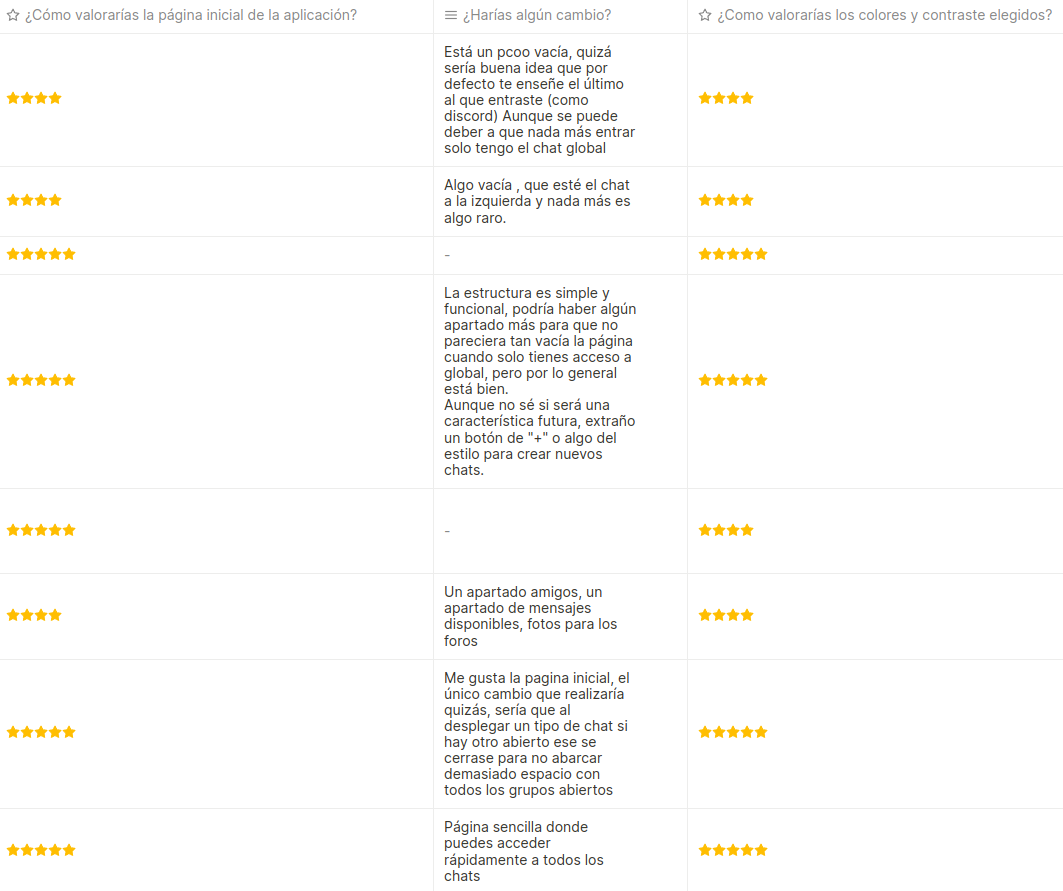
\includegraphics[width=0.9\textwidth]{res/images/resultados-encuesta-1}
		\vspace{1em}
		\hrule
		\vspace{1em}
		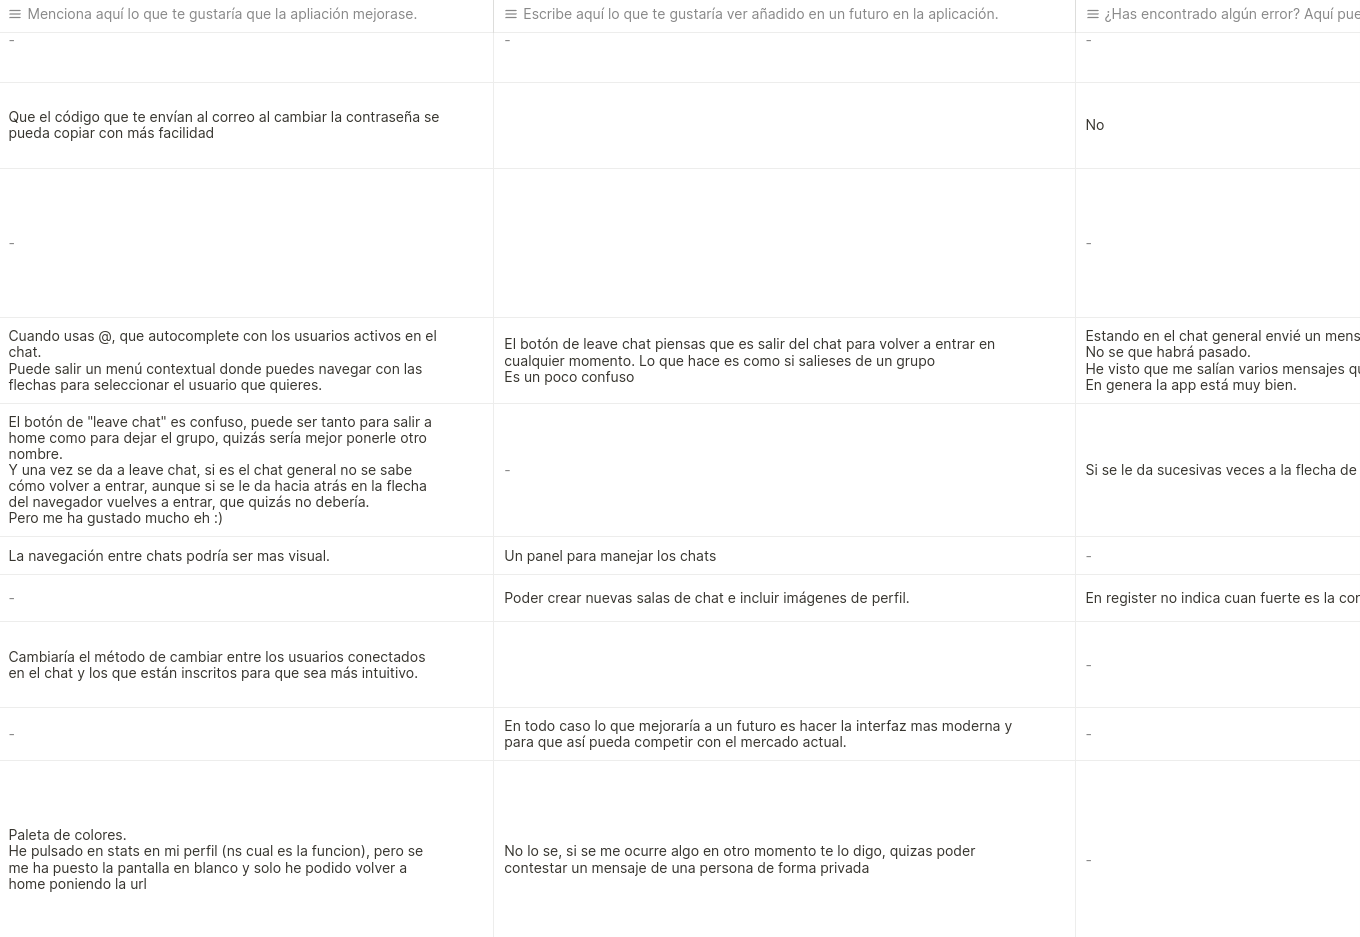
\includegraphics[width=0.9\textwidth]{res/images/resultados-encuesta-2}
		\caption{Respuestas de los usuarios a la encuesta. (Fuente: Elaboración propia).}
		\label{fig:resultados-encuesta}
	\end{figure}
\end{itemize}
